\documentclass{article}

\PassOptionsToPackage{numbers}{natbib}
\usepackage[preprint]{neurips_2026}

\usepackage[utf8]{inputenc}
\usepackage[T1]{fontenc}
\usepackage{hyperref}
\usepackage{url}
\usepackage{booktabs}
\usepackage{amsfonts}
\usepackage{amsmath}
\usepackage{amssymb}
\usepackage{nicefrac}
\usepackage{microtype}
\usepackage{xcolor}
\usepackage{graphicx}
\usepackage{enumitem}
\usepackage{subcaption}
\usepackage{multirow}

\graphicspath{{figures/}}

\title{Experimental Results: PIGNN-Attn-LS across Power System Cases}

\author{Changhun Kim}

\begin{document}
\maketitle

%==============================================================================
\section{Experimental Setup}
%==============================================================================

\subsection{Baseline Definition}

The \textbf{baseline} throughout all experiments is a \emph{flat-start}
initialisation: every bus voltage magnitude is set to $|V|=1.0$\,p.u.\ and
every voltage angle to $\theta=0^\circ$.  This is the standard cold-start
point used in classical Newton--Raphson solvers when no better estimate is
available.  The baseline RMSE and angle error reported below are the errors
of this flat-start guess against the Newton--Raphson converged solution ---
\emph{before} the model does any work.  The model's job is to reduce these
errors.

\subsection{Test Cases: Bus and Branch Counts}

Table~\ref{tab:grid_size} lists the $N_{\mathrm{bus}}$ and $N_{\mathrm{branch}}$
for each test case.  The branch count determines the number of edges in the
graph and directly affects the cost of the edge-aware attention.

\begin{table}[h]
\centering
\caption{Grid size of test cases.}
\label{tab:grid_size}
\begin{tabular}{lrrl}
\toprule
Case & $N_{\mathrm{bus}}$ & $N_{\mathrm{branch}}$ & Notes \\
\midrule
case14\_ppcY          & 14  & 20  & IEEE 14-bus \\
case24\_ieee\_rts     & 24  & 38  & IEEE RTS-24 \\
case30\_ppcY\_A       & 30  & 41  & IEEE 30-bus \\
case33bw\_ppcY\_A     & 33  & 32  & Radial distribution \\
case39\_ppcY\_A       & 39  & 46  & New England 39-bus \\
case57\_ppcY\_A       & 57  & 80  & IEEE 57-bus \\
case89pegase          & 89  & 210 & PEGASE 89-bus (dense) \\
case118\_ppcY\_A      & 118 & 186 & IEEE 118-bus \\
case145\_ppcY\_A      & 145 & 453 & PEGASE 145-bus (very dense) \\
\bottomrule
\end{tabular}
\end{table}

%==============================================================================
\section{Full Baseline vs.\ Model Comparison}
%==============================================================================

Table~\ref{tab:baseline_vs_model} summarises the RMSE of the flat-start
baseline and the trained model across all cases.  All model runs use
$K=40$, $d=4$, $d_{\mathrm{hi}}=16$, \texttt{numattn}$=1$, Armijo$=\mathrm{True}$,
100 epochs, train ratio $= 1/3$.

\begin{table}[h]
\centering
\small
\caption{Flat-start baseline vs.\ PIGNN-Attn-LS model.  Reductions are
  $\lfloor$baseline\,/\,model$\rfloor$.}
\label{tab:baseline_vs_model}
\setlength{\tabcolsep}{4pt}
\begin{tabular}{lrrrcrrc}
\toprule
\multirow{2}{*}{Case} & \multirow{2}{*}{$N_{\mathrm{bus}}$}
  & \multicolumn{2}{c}{$|V|$ RMSE (p.u.)} & \multirow{2}{*}{Reduc.}
  & \multicolumn{2}{c}{$\theta$ RMSE (${}^\circ$)} & \multirow{2}{*}{Reduc.} \\
\cmidrule(lr){3-4}\cmidrule(lr){6-7}
& & Baseline & Model & & Baseline & Model & \\
\midrule
case24\_ieee\_rts  & 24  & $2.24\times10^{-2}$ & $1\times10^{-5}$ & $\sim2000\times$ & 0.91  & 0.01 & $\sim90\times$ \\
case30\_ppcY\_A    & 30  & $1.83\times10^{-2}$ & $7\times10^{-5}$ & $\sim260\times$  & 0.21  & 0.025 & $\sim8\times$ \\
case33bw\_ppcY\_A  & 33  & $5.96\times10^{-2}$ & $5\times10^{-4}$ & $\sim120\times$  & 1.47  & 0.10  & $\sim15\times$ \\
case39\_ppcY\_A    & 39  & $1.41\times10^{-2}$ & $5\times10^{-5}$ & $\sim280\times$  & 1.50  & 0.07  & $\sim21\times$ \\
case57\_ppcY\_A    & 57  & $1.26\times10^{-1}$ & $3\times10^{-3}$ & $\sim42\times$   & 1.13  & 0.30  & $\sim4\times$ \\
case89pegase       & 89  & $2.03\times10^{-2}$ & $2.5\times10^{-3}$ & $\sim8\times$  & 0.30  & 0.27  & $\sim1.1\times$ \\
case118\_ppcY\_A   & 118 & $9.02\times10^{-3}$ & $6\times10^{-5}$ & $\sim150\times$  & 2.73  & 0.08  & $\sim34\times$ \\
case145\_ppcY\_A   & 145 & $6.52\times10^{-2}$ & $1.77\times10^{-3}$ & $\sim37\times$ & 18.64 & 1.77  & $\sim11\times$ \\
\bottomrule
\end{tabular}
\end{table}

\paragraph{Reading the baseline.}
The flat-start error is \emph{not} zero because real grids are not at
uniform $1.0\angle0^\circ$ p.u.\ at operating conditions.  The deviation
grows with grid complexity: case145 has a flat-start angle error of
$18.64^\circ$ because the PEGASE 145-bus network has strong reactive-power
variation and several high-angle buses.  case57 has a large flat-start
$|V|$ error ($0.126$\,p.u.) because it contains several buses with
voltages that differ considerably from 1.0\,p.u.\ at the operating point.

%==============================================================================
\section{Armijo vs.\ Non-Armijo}
%==============================================================================

The backtracking Armijo line search selects a step size $\alpha \in
\{1, \rho, \rho^2, \ldots\}$ at each unrolled step that satisfies the
sufficient-decrease condition on the power-mismatch $\ell^\infty$-norm:
\[
  F(x + \alpha\,\Delta x) \;\le\; (1 - c_1\,\alpha)\,F(x).
\]
Without Armijo (\texttt{armijo=False}), the full proposed step $\alpha=1$
is always accepted, which can cause oscillation or divergence when the
update overshoots.  Table~\ref{tab:armijo} shows the effect across cases.

\begin{table}[h]
\centering
\caption{Effect of Armijo line search. $K=40$, $d=4$, $d_{\mathrm{hi}}=16$,
  \texttt{numattn}$=1$, 100\,ep.}
\label{tab:armijo}
\begin{tabular}{lrrrrl}
\toprule
\multirow{2}{*}{Case} & \multicolumn{2}{c}{Without Armijo} & \multicolumn{2}{c}{With Armijo} & \multirow{2}{*}{Verdict} \\
\cmidrule(lr){2-3}\cmidrule(lr){4-5}
& $|V|$ RMSE & $\theta$ (${}^\circ$) & $|V|$ RMSE & $\theta$ (${}^\circ$) & \\
\midrule
case24\_ieee\_rts & $6\times10^{-4}$ & 0.025 & $\mathbf{1\times10^{-5}}$ & $\mathbf{0.01}$ & Large gain \\
case30\_ppcY\_A   & $3\times10^{-4}$ & 0.20  & $\mathbf{7\times10^{-5}}$ & $\mathbf{0.025}$ & Large gain \\
case33bw\_ppcY\_A & $1.5\times10^{-3}$ & 0.10 & $5\times10^{-4}$ & 0.10 & Modest gain \\
case39\_ppcY\_A   & $5\times10^{-3}$ & 0.10  & $\mathbf{5\times10^{-5}}$ & $\mathbf{0.07}$ & Large gain \\
case57\_ppcY\_A   & $3\times10^{-3}$ & 0.20  & $3\times10^{-3}$ & 0.30 & No gain \\
case89pegase      & $3\times10^{-3}$ & 0.30  & $2.5\times10^{-3}$ & 0.27 & Marginal \\
case118\_ppcY\_A  & $4\times10^{-4}$ & 0.09  & $\mathbf{6\times10^{-5}}$ & $\mathbf{0.08}$ & Large gain \\
case145\_ppcY\_A  & $0.010$ & 6.0   & $3\times10^{-3}$ & 6.0  & Modest gain \\
\bottomrule
\end{tabular}
\end{table}

For most cases, Armijo produces a significant accuracy improvement by
preventing divergent updates.  The exceptions are case57 and case89pegase,
which appear to be architecturally undersized at ($K=40$, $d_{\mathrm{hi}}=16$):
both cases plateau regardless of the step-size policy.  case89pegase is
notably dense ($N_{\mathrm{branch}}=210$ for 89 buses), which may
require a larger model.

\subsection{Representative Learning Curves}

Figures~\ref{fig:armijo_24}--\ref{fig:armijo_145} show the validation RMSE
curves ($|V|$ and $\theta$) for four representative cases, contrasting
Armijo=False and Armijo=True.

\begin{figure}[h]
  \centering
  \begin{subfigure}[b]{0.48\textwidth}
    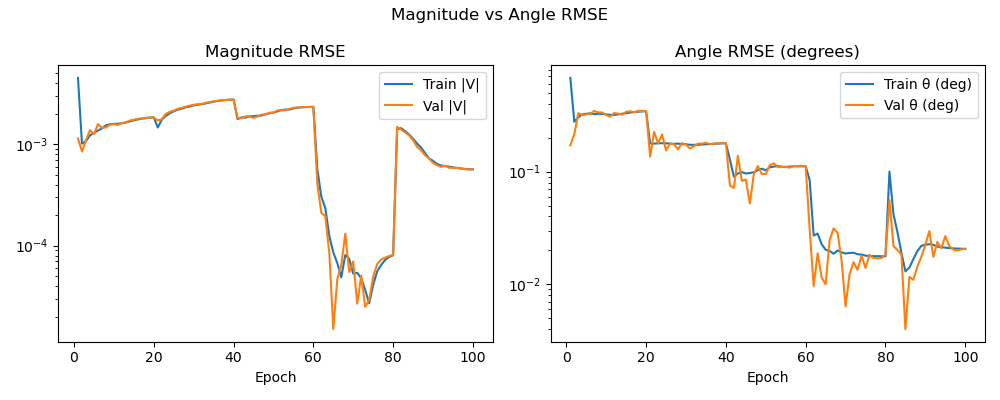
\includegraphics[width=\textwidth]{case24_ieee_rts_armijoFalse_rmse}
    \caption{case24 -- Armijo=False}
  \end{subfigure}
  \hfill
  \begin{subfigure}[b]{0.48\textwidth}
    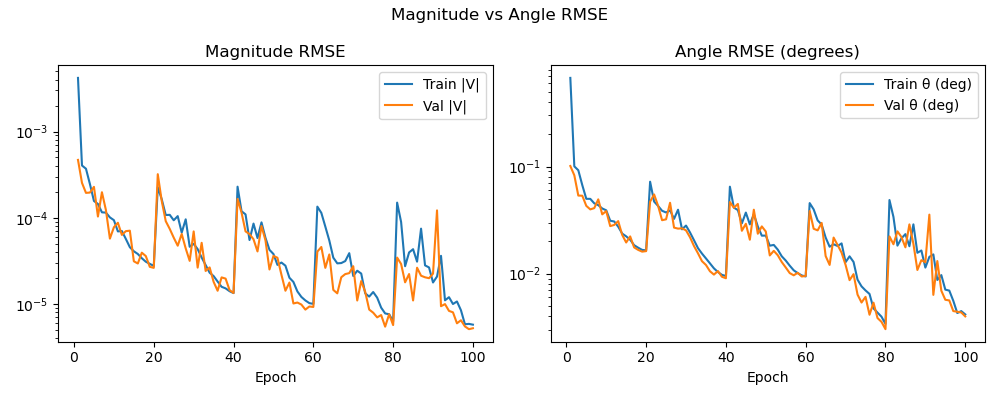
\includegraphics[width=\textwidth]{case24_ieee_rts_armijoTrue_rmse}
    \caption{case24 -- Armijo=True}
  \end{subfigure}
  \caption{case24\_ieee\_rts: Armijo reduces $|V|$ RMSE by $\sim60\times$
    and stabilises training.}
  \label{fig:armijo_24}
\end{figure}

\begin{figure}[h]
  \centering
  \begin{subfigure}[b]{0.48\textwidth}
    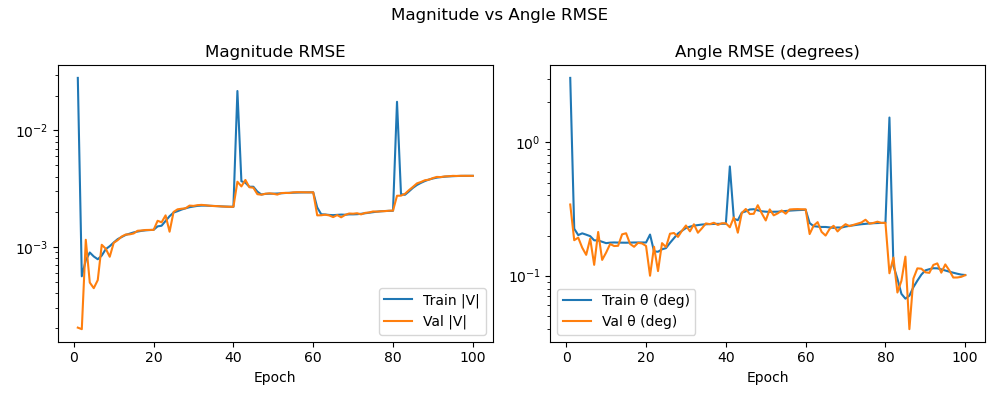
\includegraphics[width=\textwidth]{case39_ppcY_A_armijoFalse_rmse}
    \caption{case39 -- Armijo=False (diverges)}
  \end{subfigure}
  \hfill
  \begin{subfigure}[b]{0.48\textwidth}
    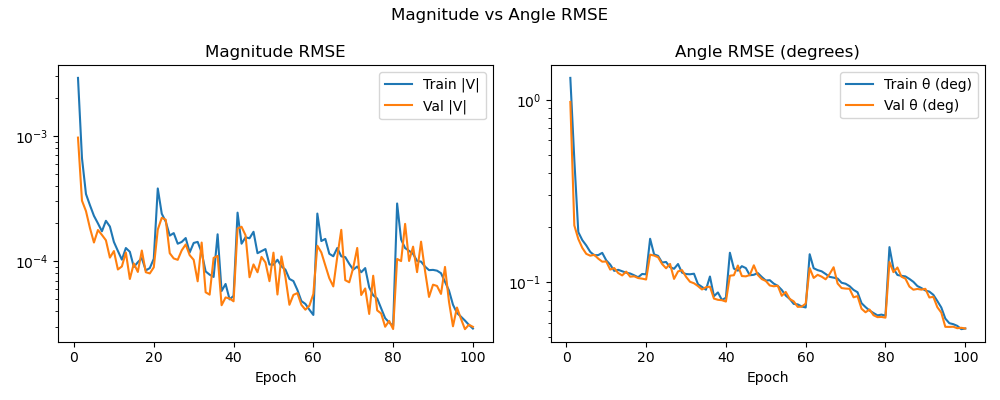
\includegraphics[width=\textwidth]{case39_ppcY_A_armijoTrue_rmse}
    \caption{case39 -- Armijo=True (converges)}
  \end{subfigure}
  \caption{case39\_ppcY\_A: without Armijo the updates overshoot and
    diverge; Armijo restores stable descent.}
  \label{fig:armijo_39}
\end{figure}

\begin{figure}[h]
  \centering
  \begin{subfigure}[b]{0.48\textwidth}
    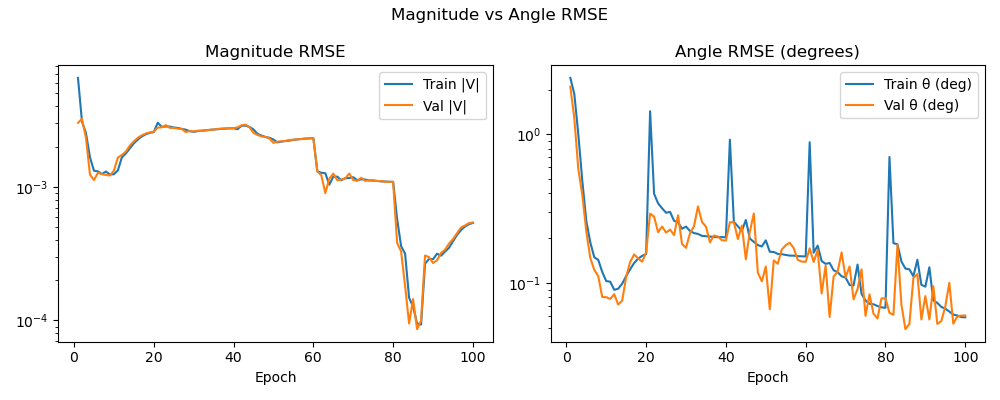
\includegraphics[width=\textwidth]{case118_ppcY_A_armijoFalse_rmse}
    \caption{case118 -- Armijo=False}
  \end{subfigure}
  \hfill
  \begin{subfigure}[b]{0.48\textwidth}
    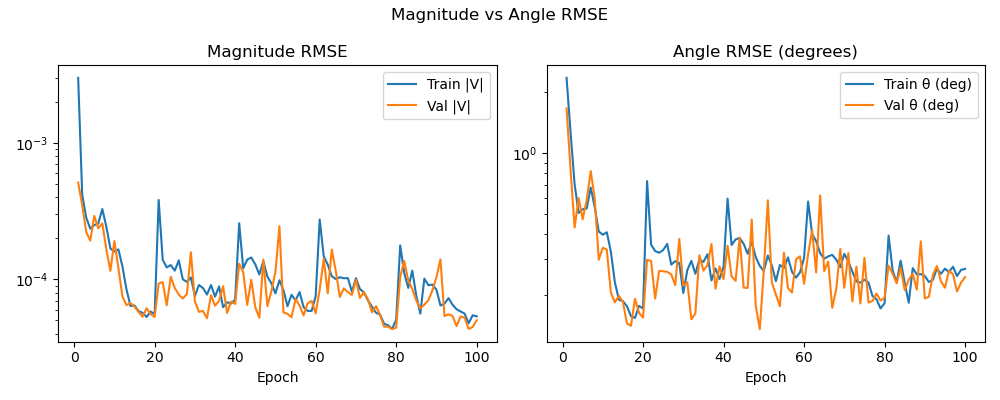
\includegraphics[width=\textwidth]{case118_ppcY_A_armijoTrue_rmse}
    \caption{case118 -- Armijo=True}
  \end{subfigure}
  \caption{case118\_ppcY\_A: Armijo reduces $|V|$ RMSE by $\sim7\times$
    and produces a sawtooth descent pattern consistent with cosine-restart
    scheduling.}
  \label{fig:armijo_118}
\end{figure}

\begin{figure}[h]
  \centering
  \begin{subfigure}[b]{0.48\textwidth}
    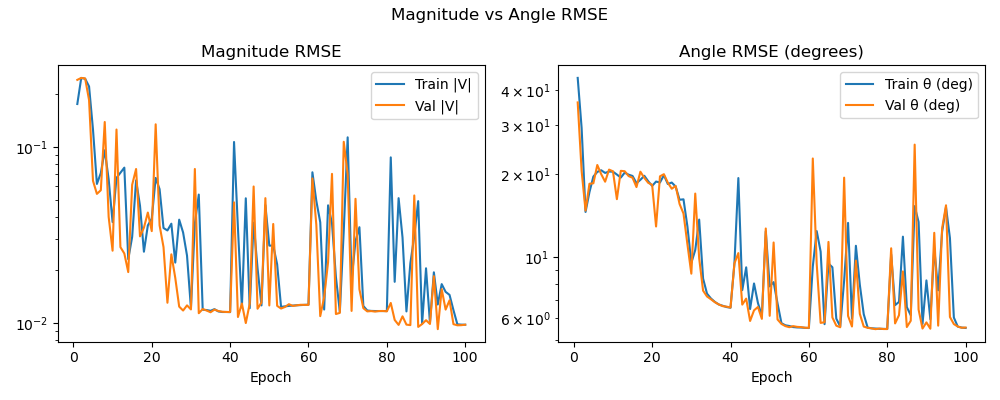
\includegraphics[width=\textwidth]{case145_ppcY_A_armijoFalse_rmse}
    \caption{case145 -- Armijo=False (oscillates)}
  \end{subfigure}
  \hfill
  \begin{subfigure}[b]{0.48\textwidth}
    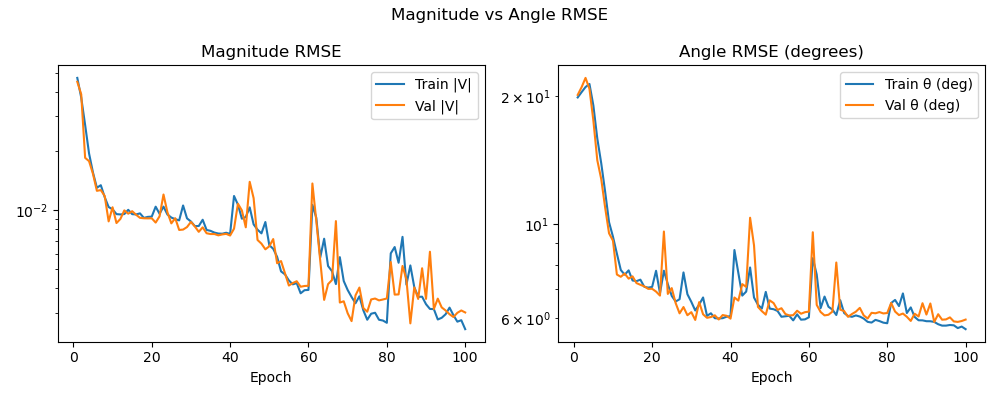
\includegraphics[width=\textwidth]{case145_ppcY_A_armijoTrue_rmse}
    \caption{case145 -- Armijo=True (smoother)}
  \end{subfigure}
  \caption{case145\_ppcY\_A (small config, $d_{\mathrm{hi}}=16$, \texttt{numattn}$=1$):
    Armijo reduces $|V|$ RMSE by $\sim3\times$ but $\theta$ RMSE stays
    near $6^\circ$, indicating the model is undersized for this case.}
  \label{fig:armijo_145}
\end{figure}

%==============================================================================
\section{case145 Architecture Sweep}
%==============================================================================

\subsection{What is the Pareto Front?}

In a multi-objective setting, a run is \textbf{Pareto-optimal} (or
Pareto-dominant) if no other run is \emph{strictly better on every
objective simultaneously}.  Here the two objectives are:
\begin{enumerate}[noitemsep]
  \item Minimise $|V|$ RMSE (voltage magnitude accuracy).
  \item Minimise $\theta$ RMSE (angle accuracy).
\end{enumerate}
A run is on the Pareto front if you cannot improve one metric without
making the other worse.  Pareto-optimal runs represent the
\emph{accuracy--accuracy} trade-off frontier and are the natural
candidates for deployment depending on which metric the operator
prioritises.

\subsection{Part~A: Launcher Log Sweep}

All runs: $K=40$, 100\,epochs, Armijo$=\mathrm{False}$.
Sorted by $\theta$ RMSE (best first).
Runs with $d_{\mathrm{hi}}=64$ diverged catastrophically (physics loss
$\sim10^5$) and are listed separately.  The OOM run is excluded.

\begin{table}[h]
\centering
\scriptsize
\caption{case145 architecture sweep (launcher log sweep).
  $\checkmark$ = Pareto-optimal. $H$=heads, $L$=attn layers.}
\label{tab:case145_sweep}
\setlength{\tabcolsep}{3pt}
\begin{tabular}{clrrrrrrrrl}
\toprule
Rank & Label & $H$ & $d_{\mathrm{hi}}$ & $L$ & Params
  & $\mathcal{L}_{\mathrm{phys}}$ & $|V|$ RMSE & $\theta$ (${}^\circ$)
  & $\Delta P^\infty$ & Pareto \\
\midrule
1  & 03\_nhead8\_dhi24\_attn8   & 8 & 24 & 8  & 65,896  & 0.426 & $1.767\times10^{-3}$ & \textbf{1.770} & 2.750 & $\checkmark$ \\
2  & 09\_nhead8\_dhi32\_attn10  & 8 & 32 & 10 & 137,288 & 0.498 & $2.758\times10^{-3}$ & 2.440 & \textbf{0.320} & \\
3  & 04\_nhead8\_dhi24\_attn10  & 8 & 24 & 10 & 80,816  & 0.461 & $4.140\times10^{-3}$ & 2.776 & 0.457 & \\
4  & 08\_nhead8\_dhi32\_attn8   & 8 & 32 & 8  & 111,472 & 0.458 & $6.323\times10^{-3}$ & 2.824 & 0.990 & \\
5  & 16\_nhead12\_dhi24\_attn4  & 12& 24 & 4  & 36,360  & 0.503 & $\mathbf{1.213\times10^{-3}}$ & 3.973 & 3.374 & $\checkmark$ \\
6  & 17\_nhead12\_dhi24\_attn6  & 12& 24 & 6  & 51,432  & 0.461 & $5.496\times10^{-3}$ & 4.012 & 5.520 & \\
7  & 05\_nhead8\_dhi24\_attn12  & 8 & 24 & 12 & 95,736  & 0.431 & $3.472\times10^{-2}$ & 4.075 & 1.778 & \\
8  & 18\_nhead12\_dhi24\_attn8  & 12& 24 & 8  & 66,504  & 0.836 & $2.324\times10^{-2}$ & 4.794 & 1.114 & \\
9  & 01\_nhead8\_dhi24\_attn4   & 8 & 24 & 4  & 36,056  & 0.473 & $1.671\times10^{-3}$ & 4.945 & 1.148 & $\checkmark$ \\
10 & 06\_nhead8\_dhi32\_attn4   & 8 & 32 & 4  & 59,840  & 0.493 & $2.622\times10^{-2}$ & 5.079 & 1.350 & \\
11 & 02\_nhead8\_dhi24\_attn6   & 8 & 24 & 6  & 50,976  & 0.446 & $4.395\times10^{-3}$ & 5.411 & 4.612 & \\
12 & 07\_nhead8\_dhi32\_attn6   & 8 & 32 & 6  & 85,656  & 0.513 & $3.259\times10^{-3}$ & 6.354 & 9.195 & \\
\midrule
OOM  & 10\_nhead8\_dhi32\_attn12 & 8 & 32 & 12 & 163,104 & \multicolumn{5}{c}{out of memory} \\
FAIL & 11\_nhead8\_dhi64\_attn4  & 8 & 64 & 4 & 216,416 & $1.51\times10^5$ & 0.246 & $39.6^\circ$ & 490 & diverged \\
FAIL & 12\_nhead8\_dhi64\_attn6  & 8 & 64 & 6 & 316,536 & $1.66\times10^5$ & 0.241 & $88.0^\circ$ & 729 & diverged \\
\midrule
--- & runs 19--45 & \multicolumn{9}{c}{nhead=12 ($d_{\mathrm{hi}}\ge48$), nhead=16 -- incomplete} \\
\bottomrule
\end{tabular}
\end{table}

The three Pareto-optimal runs are:
\begin{itemize}[noitemsep]
  \item \textbf{Rank 1} ($H=8$, $d_{\mathrm{hi}}=24$, $L=8$, 65k params):
    best $\theta$ at $1.77^\circ$.
  \item \textbf{Rank 5} ($H=12$, $d_{\mathrm{hi}}=24$, $L=4$, 36k params):
    best $|V|$ RMSE at $1.21\times10^{-3}$, smallest Pareto model.
  \item \textbf{Rank 9} ($H=8$, $d_{\mathrm{hi}}=24$, $L=4$, 36k params):
    good $|V|$ RMSE ($1.67\times10^{-3}$) at minimal cost; also 36k params
    but worse than Rank 5 on $|V|$.
\end{itemize}

\begin{figure}[h]
  \centering
  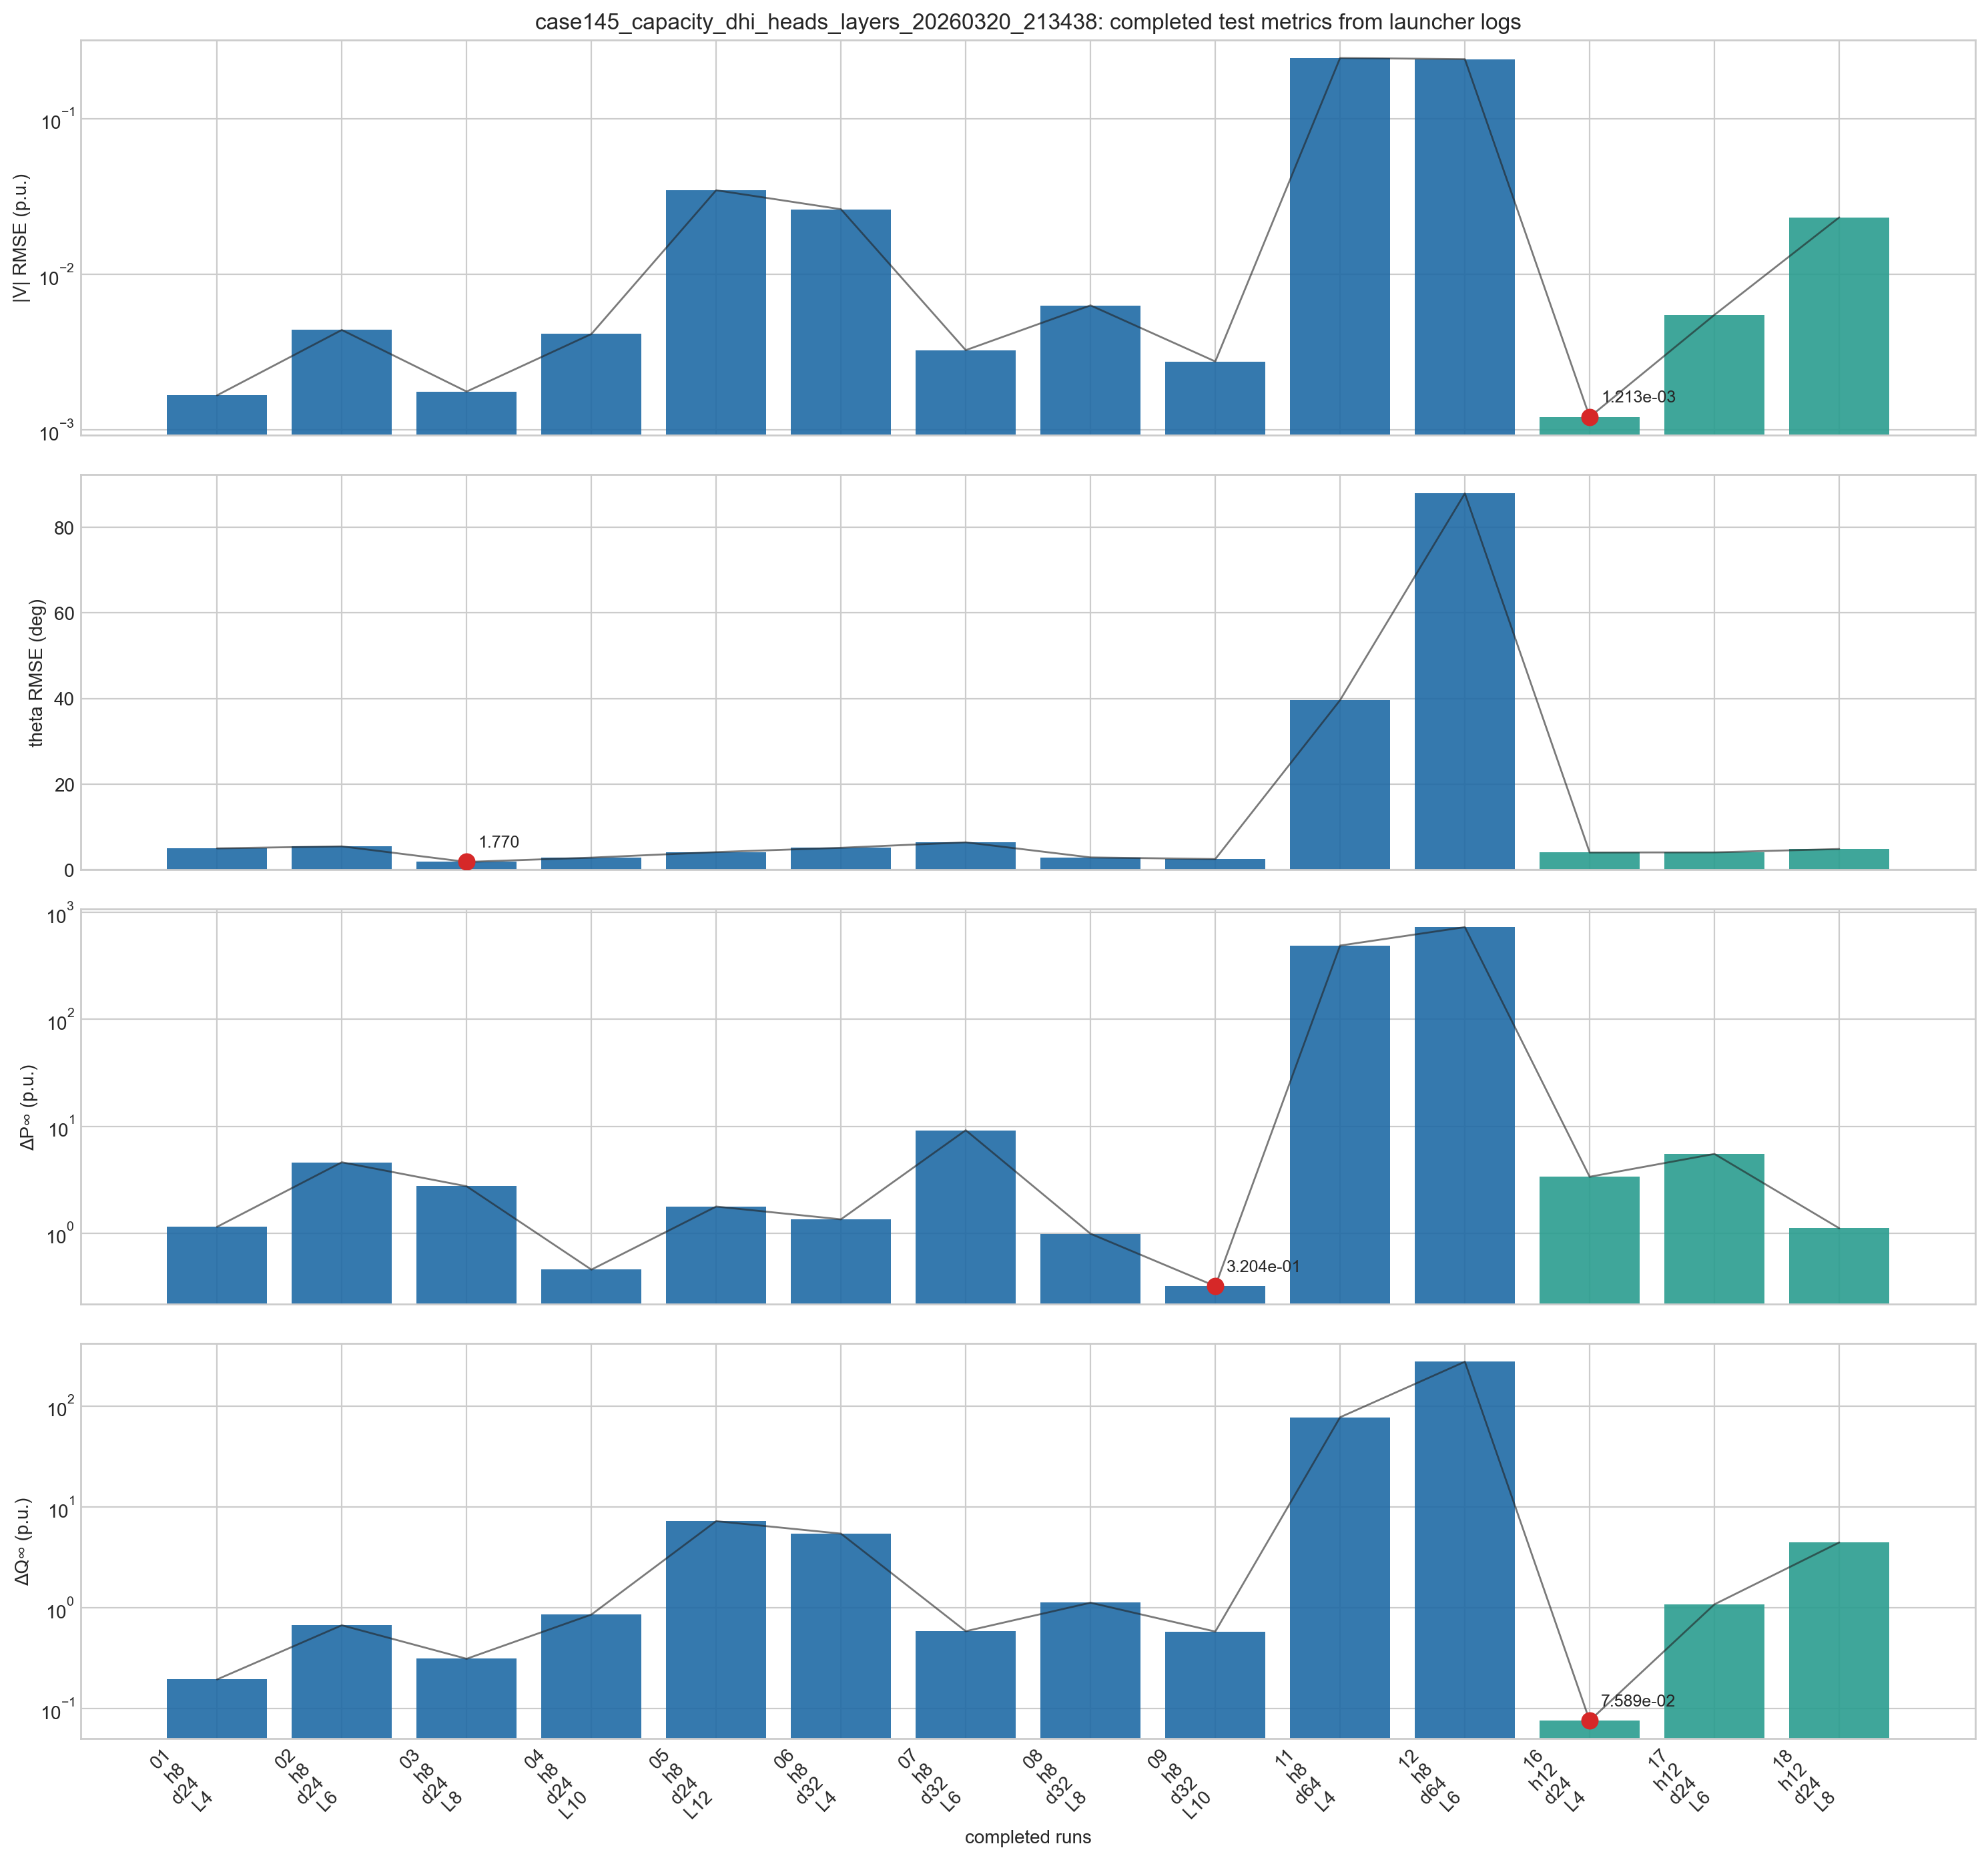
\includegraphics[width=0.85\textwidth]{case145_sweep_metrics}
  \caption{case145 launcher sweep: test metrics by run
    ($K=40$, Armijo=False).  Pareto-optimal runs are the best in the
    lower-left of the $|V|$--$\theta$ plane.}
  \label{fig:sweep}
\end{figure}

\subsection{Part~B: Earlier Plot-Based Runs (small configs, numattn $= 1$--$2$)}

These runs predate the full sweep and used smaller $d_{\mathrm{hi}}$ and
fewer attention layers.

\begin{table}[h]
\centering
\caption{case145 earlier runs (from validation learning curves).}
\label{tab:case145_early}
\begin{tabular}{lrrrrrrl}
\toprule
Config & $K$ & $d$ & $d_{\mathrm{hi}}$ & \texttt{numattn} & Armijo
  & $|V|$ RMSE & $\theta$ (${}^\circ$) \\
\midrule
K40\_d4\_dhi16\_n1 & 40 & 4 & 16 & 1 & False & $\sim0.010$      & $\sim6$ \\
K40\_d4\_dhi16\_n1 & 40 & 4 & 16 & 1 & \textbf{True}  & $\sim3\times10^{-3}$ & $\sim6$ \\
K40\_d4\_dhi16\_n2 & 40 & 4 & 16 & 2 & False & $\sim2\times10^{-3}$ & $\sim5$ \\
K40\_d4\_dhi24\_n1 & 40 & 4 & 24 & 1 & False & $\sim0.010$      & $\sim5$ \\
K40\_d4\_dhi24\_n2 & 40 & 4 & 24 & 2 & False & $\sim8\times10^{-3}$ & $\sim5$ \\
K40\_d6\_dhi16\_n1 & 40 & 6 & 16 & 1 & False & $\sim0.030$      & $\sim6$ \\
K40\_d6\_dhi24\_n1 & 40 & 6 & 24 & 1 & False & $\sim0.015$      & $\sim5$ \\
K48\_d4\_dhi16\_n1 & 48 & 4 & 16 & 1 & False & $\sim3\times10^{-3}$ & $\sim5$ \\
K48\_d4\_dhi24\_n2 & 48 & 4 & 24 & 2 & False & $\sim3\times10^{-3}$ & $\sim5$ \\
K48\_d6\_dhi24\_n2 & 48 & 6 & 24 & 2 & False & $\sim0.010$      & $\sim10$ \\
\bottomrule
\end{tabular}
\end{table}

\begin{figure}[h]
  \centering
  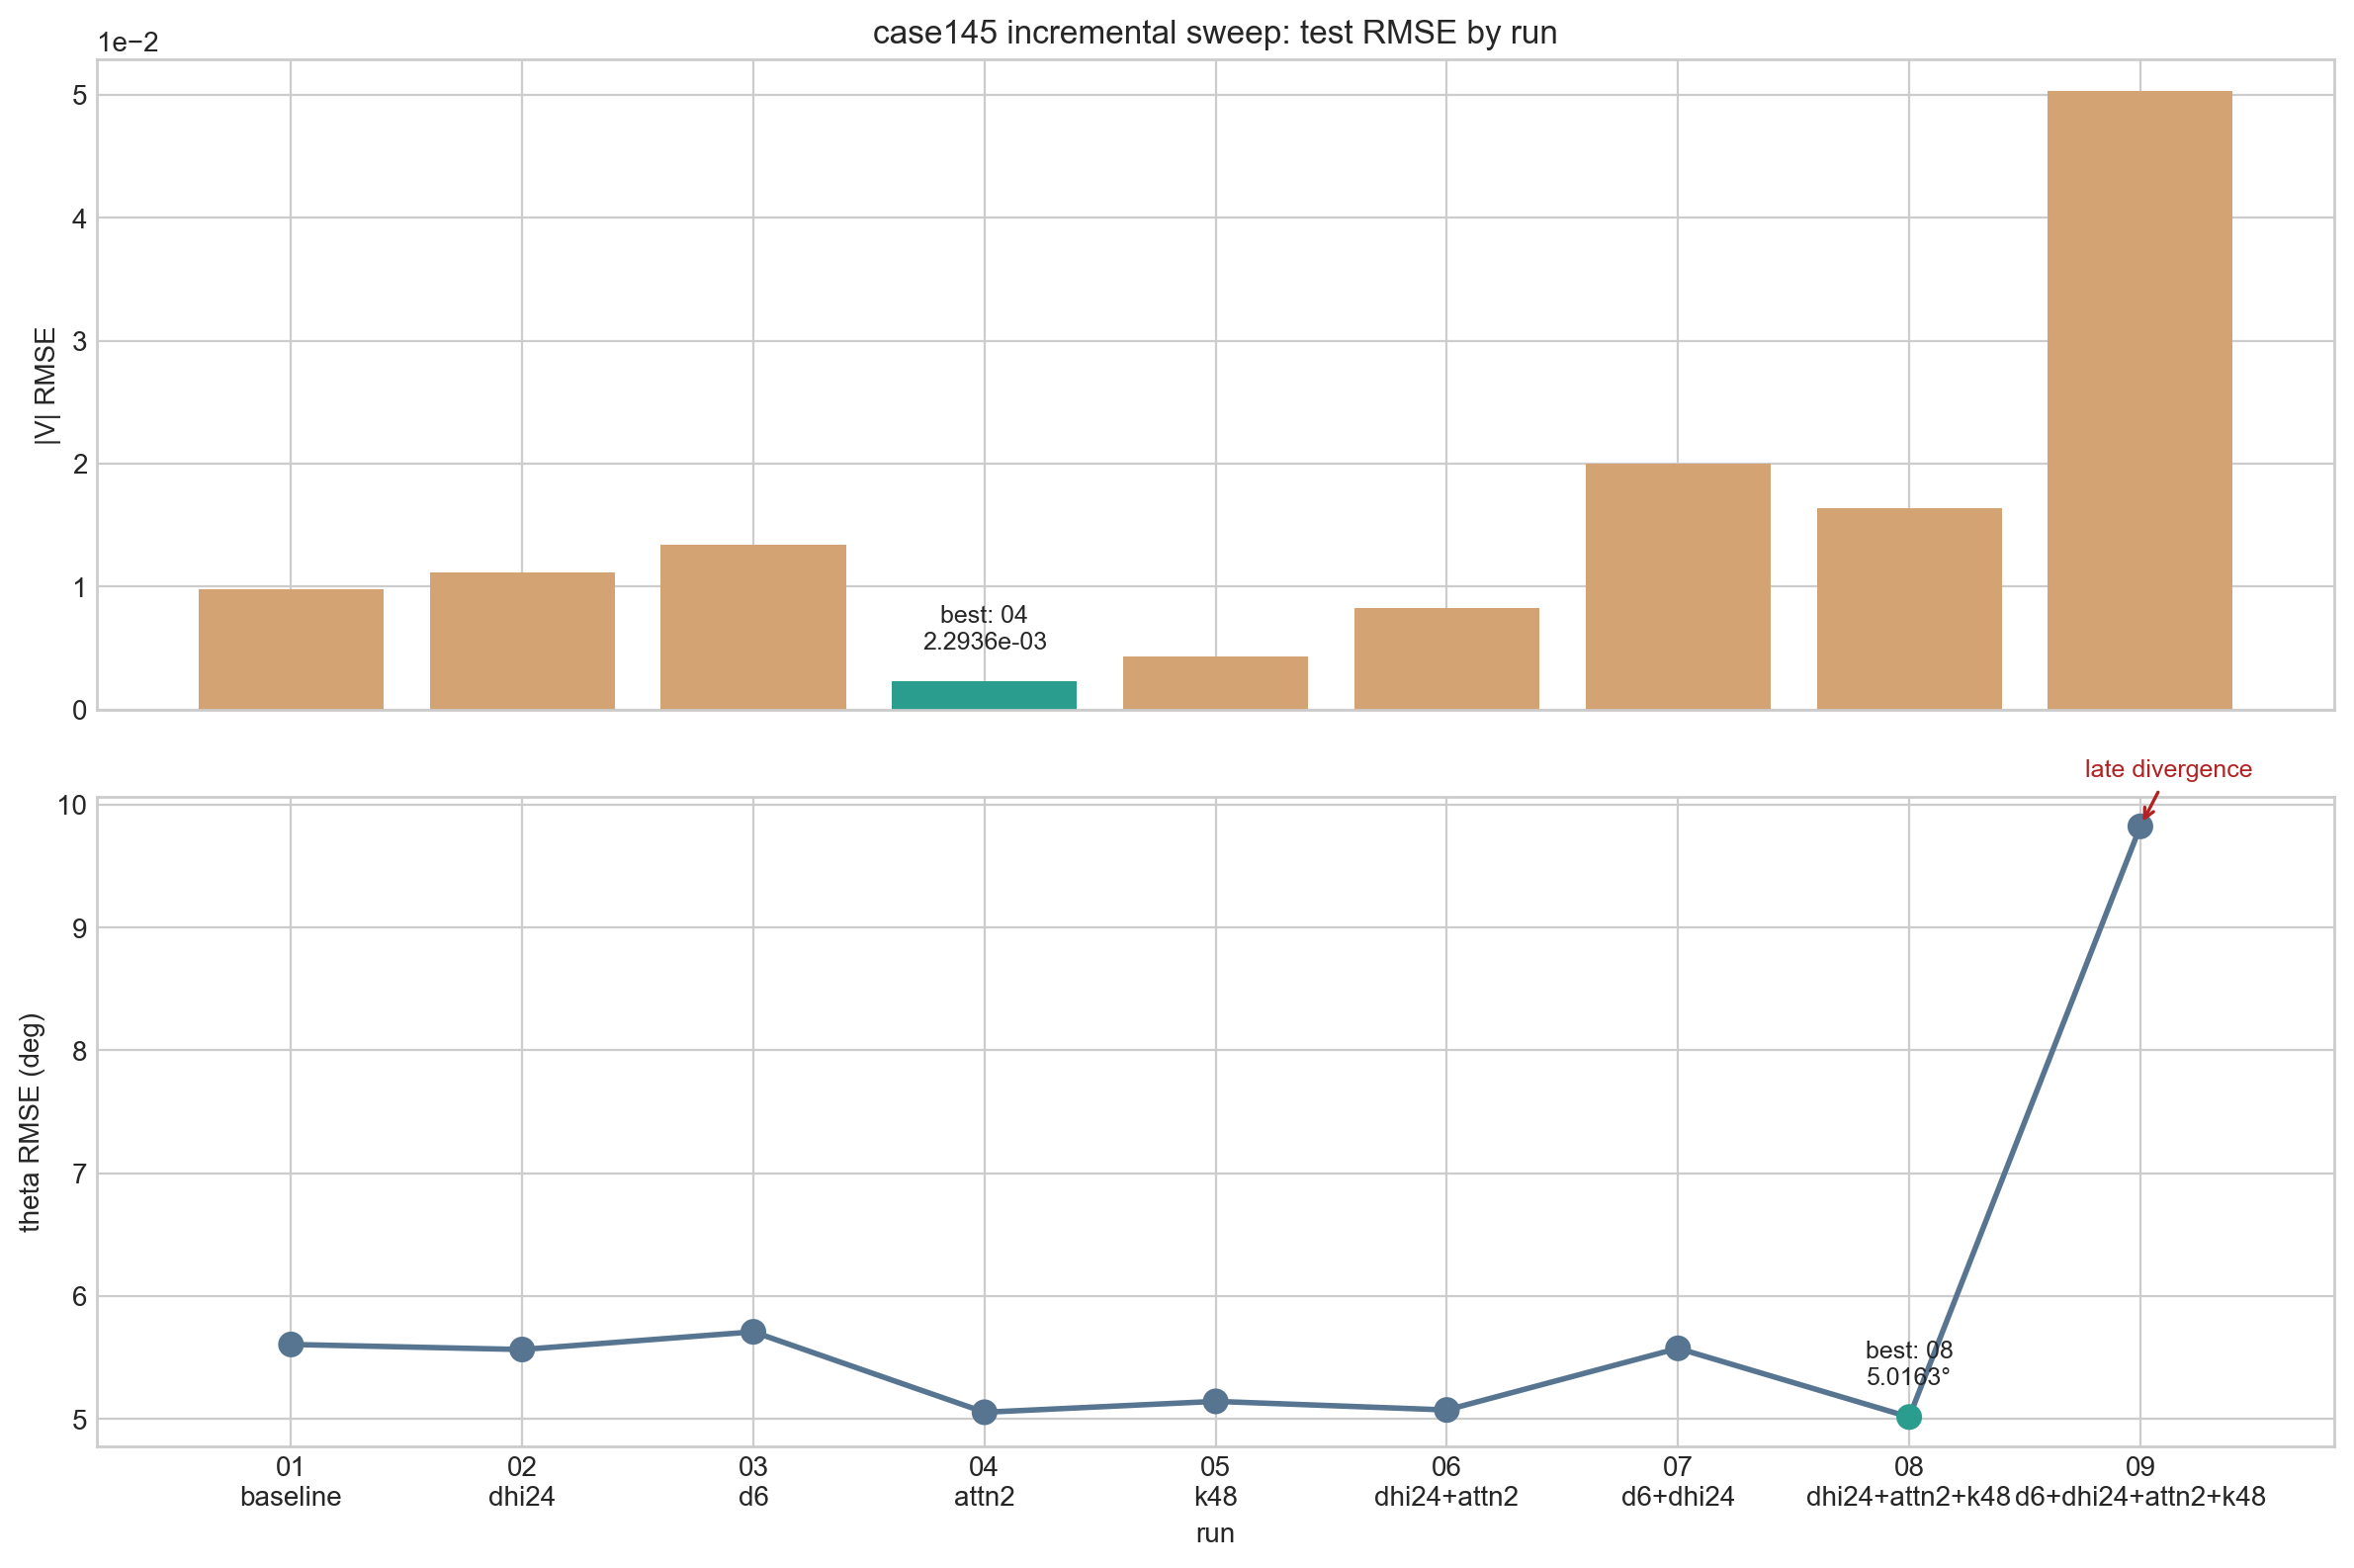
\includegraphics[width=0.75\textwidth]{case145_incremental}
  \caption{case145 incremental run summary (earlier small-config sweep).
    All configs plateau at $\theta \approx 5$--$6^\circ$, well above the
    best from the full capacity sweep ($1.77^\circ$).}
  \label{fig:incremental}
\end{figure}

\subsection{Key Findings}

\begin{enumerate}[noitemsep]
  \item \textbf{Best overall:} $H{=}8$, $d_{\mathrm{hi}}{=}24$, $L{=}8$
    (65k params) achieves $\theta = 1.77^\circ$, $|V| = 1.77\times10^{-3}$.
  \item \textbf{Best $|V|$ RMSE:} $H{=}12$, $d_{\mathrm{hi}}{=}24$, $L{=}4$
    (36k params) achieves $|V| = 1.21\times10^{-3}$, but $\theta = 3.97^\circ$.
  \item \textbf{Deeper is not always better:} for $d_{\mathrm{hi}}=24$,
    $L{=}8$ outperforms both $L{=}10$ and $L{=}12$ on angle accuracy.
    $L{=}12$ has 3$\times$ the angle RMSE of $L{=}8$.
  \item \textbf{$d_{\mathrm{hi}}=64$ diverged completely:} physics loss jumped
    to $\sim10^5$, $\theta$ errors of $40$--$88^\circ$.  The likely cause
    is that the large hidden dimension magnifies gradient variance at
    initialisation (all heads initialised to zero), making the early
    training unstable under the physics loss only.
  \item \textbf{Small configs plateau at $\theta \approx 5$--$6^\circ$:}
    the earlier runs with $d_{\mathrm{hi}} \le 16$ and \texttt{numattn}$\le2$
    all converge to this plateau, confirming that architectural capacity
    (not just steps $K$) is the bottleneck for case145.
  \item \textbf{Many sweep runs still incomplete:} nhead$=12$ with
    $d_{\mathrm{hi}}\ge48$ and all nhead$=16$ runs are pending; better
    configurations may yet be found.
\end{enumerate}

\end{document}
